% Drawing 74/04-10 -- folder 74, batch 04, archive page 77 (PDF page 78).
% Transcription: grand diagramme de revêtements, flèches marquées 2 ou 3, entre : « hex + diag $\simeq$ tria + él. marqué $\simeq$ couples de triades \uncertain{séquentes} (\uncertain{explicites}) » ; « $\mathrm{tria}' = \mathrm{Hex} + \mathrm{diag}$, $\mathrm{Hex} + \mathrm{codiag} = \mathrm{bib.\,plié}$ » ; « $\mathrm{tria} \simeq \mathrm{hex} = \mathrm{Hex} + \text{sommet}$ » (flèche « opp ») ; « hex or (hex + orientation) $\simeq$ tria or (triade + ordre circulaire) $\simeq \omega((\mathrm{hex+diag})/\mathrm{hex})$ » ; « $\mathrm{Hex}$ » ; « $\mathrm{trtria} \simeq \omega(\mathrm{Hex}/\mathrm{triHex}) \simeq$ Hex + triangle inscrit $\simeq$ pavé orienté » ; « hex + sommet » ; « hex + triangle inscrit orienté $\simeq$ couple de triades orientées parallèles » ; « $\mathrm{Hex} + \mathrm{rep} \simeq$ couple de triades liées $\simeq$ couple de triades par. $\simeq$ hex + triade marquée $\simeq$ hex + triangle inscrit » avec les mentions « torseur sous Hex de groupe $\mathfrak{S}_3 \times \mathfrak{S}_2$ », « torseur sur trtria de groupe $\mathfrak{S}_3$ », « torseur sur tria de groupe $\mathfrak{S}_2$ » ; « $\mathrm{tria}' = \mathrm{Hex} + \mathrm{rep\ mod\ opp}$ (torseur sur Hex de groupe $\mathfrak{S}_3$) » ; « $\mathrm{triHex}$ », « $\mathrm{triHex}$ » (doublé) ; « $\mathrm{Hexor} = \omega(\mathrm{tri}'/\mathrm{Hex}) = \mathrm{Hex} + \mathrm{or}$ » ; « dror tria $\simeq$ Hex + dr.\ or.\ \uncertain{inscr.} ». En bas, un cube des ensembles $H_s$, $H_r$, $H_{p'}$, $H_{s^*}$, $H_d$, $H_{tr}$, $H_{trr}$, $H_\omega$, $H_{tr^*}$, $e$, marqué $\mathfrak{S}_3 \times \mathfrak{S}_2$, avec de petits hexagones dessinés à côté.
% Kind: large diagram of coverings, cube of sets H_*, small hexagons. Method 2 (schematic redraw from the facsimile). Status: partial.
% Notes: Landscape sheet. Each node is placed where it stands, with its label shortened to its first identification (the full labels are in the transcription); arrows as seen with their degree 2 or 3 and the « opp » marks. Many arrows cross and some of their ends are a reading. The cube of the sets H_s ... e at the lower right is drawn schematically (labels as the transcription gives them; their exact positions in the overinked cube are approximate), with S_3 x S_2 beside it; the small hexagons are drawn as outlines. The list « H un hexagone, H_d ensemble des diagonales ... » at the upper right and the lists of pairs at the upper left are text and are not drawn.
% Coordinates: 1 unit = 1 mm = 1/100 of the crop width (bbox in page fractions: [0.08, 0.05, 0.95, 0.52]).
% Redrawn by Claude (claude-opus-5-5), issue #73, 2026-11-07; not checked by a human; not compiled (no TeX in the session).
% Rights: reproduces part of the work -- behind RENDER_TRANSCRIPTS, never published by itself.
\documentclass[tikz,border=3pt]{standalone}
\usepackage{amsmath,amssymb}
\usetikzlibrary{patterns,arrows.meta}
\tikzset{pencil/.style={black!45}, struck/.style={black!35}, mark/.style={circle,draw,inner sep=1.3pt}, pt/.style={circle,fill,inner sep=0.9pt}, opt/.style={circle,draw,fill=white,inner sep=1.1pt}}
\begin{document}
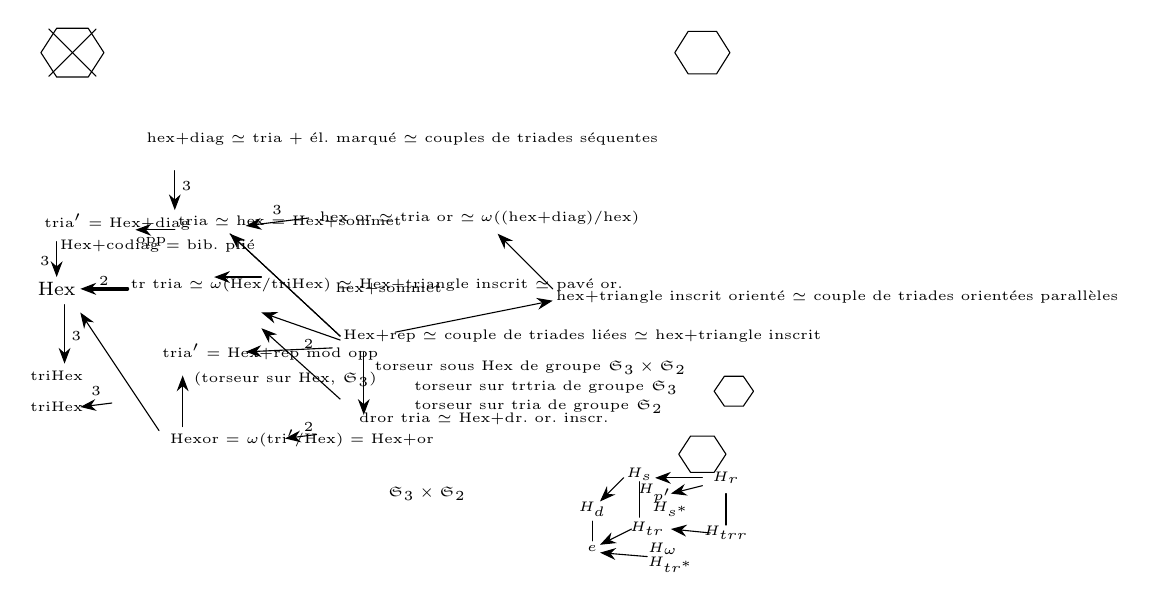
\begin{tikzpicture}[x=1mm,y=1mm,line cap=round,line join=round,font=\scriptsize]
\node[inner sep=1pt,anchor=west] at (22,-21) {\tiny hex$+$diag $\simeq$ tria $+$ él.\ marqué $\simeq$ couples de triades séquentes};
\draw[-{Stealth[length=2mm]}] (26,-25) -- (26,-30);
\node[inner sep=1pt] at (27.5,-27) {\tiny $3$};
\node[inner sep=1pt,anchor=west] at (9,-31.5) {\tiny tria$'$ = Hex$+$diag};
\node[inner sep=1pt,anchor=west] at (11,-34.5) {\tiny Hex$+$codiag = bib.\ plié};
\node[inner sep=1pt,anchor=west] at (26,-31.5) {\tiny tria $\simeq$ hex = Hex$+$sommet};
\draw[-{Stealth[length=2mm]}] (26,-32.5) -- (21,-32.5);
\node[inner sep=1pt] at (23,-34) {\tiny opp};
\node[inner sep=1pt,anchor=west] at (44,-31) {\tiny hex or $\simeq$ tria or $\simeq\omega$((hex$+$diag)/hex)};
\draw[-{Stealth[length=2mm]}] (43,-31) -- (35,-32);
\node[inner sep=1pt] at (39,-30) {\tiny $3$};
\node[inner sep=1pt] at (11,-40) {\scriptsize Hex};
\draw[-{Stealth[length=2mm]}] (11,-34) -- (11,-38.5);
\node[inner sep=1pt] at (9.5,-36.5) {\tiny $3$};
\node[inner sep=1pt,anchor=west] at (20,-39.5) {\tiny tr tria $\simeq\omega$(Hex/triHex) $\simeq$ Hex$+$triangle inscrit $\simeq$ pavé or.};
\draw[-{Stealth[length=2mm]},very thick] (20,-40) -- (14,-40);
\node[inner sep=1pt] at (17,-39) {\tiny $2$};
\node[inner sep=1pt,anchor=west] at (46,-40) {\tiny hex$+$sommet};
\draw[-{Stealth[length=2mm]}] (37,-38.5) -- (31,-38.5);
\node[inner sep=1pt,anchor=west] at (74,-41) {\tiny hex$+$triangle inscrit orienté $\simeq$ couple de triades orientées parallèles};
\draw[-{Stealth[length=2mm]}] (74,-40) -- (67,-33);
\node[inner sep=1pt,anchor=west] at (47,-46) {\tiny Hex$+$rep $\simeq$ couple de triades liées $\simeq$ hex$+$triangle inscrit};
\node[inner sep=1pt,anchor=west] at (51,-50) {\tiny torseur sous Hex de groupe $\mathfrak S_3\times\mathfrak S_2$};
\node[inner sep=1pt,anchor=west] at (56,-52.5) {\tiny torseur sur trtria de groupe $\mathfrak S_3$};
\node[inner sep=1pt,anchor=west] at (56,-55) {\tiny torseur sur tria de groupe $\mathfrak S_2$};
\draw[-{Stealth[length=2mm]}] (47,-46) -- (33,-33);
\draw[-{Stealth[length=2mm]}] (47,-46.5) -- (37,-43);
\draw[-{Stealth[length=2mm]}] (46,-47.5) -- (35,-48);
\node[inner sep=1pt] at (43,-47) {\tiny $2$};
\draw[-{Stealth[length=2mm]}] (54,-45.5) -- (74,-41.5);
\draw[-{Stealth[length=2mm]}] (50,-48) -- (50,-56);
\node[inner sep=1pt,anchor=west] at (24,-48) {\tiny tria$'$ = Hex$+$rep mod opp};
\node[inner sep=1pt,anchor=west] at (28,-51.5) {\tiny (torseur sur Hex, $\mathfrak S_3$)};
\node[inner sep=1pt] at (11,-51) {\tiny triHex};
\node[inner sep=1pt] at (11,-55) {\tiny triHex};
\draw[-{Stealth[length=2mm]}] (18,-54.5) -- (14,-55);
\node[inner sep=1pt] at (16,-53) {\tiny $3$};
\draw[-{Stealth[length=2mm]}] (12,-42) -- (12,-49.5);
\node[inner sep=1pt] at (13.5,-46) {\tiny $3$};
\node[inner sep=1pt,anchor=west] at (25,-59) {\tiny Hexor = $\omega$(tri$'$/Hex) = Hex$+$or};
\draw[-{Stealth[length=2mm]}] (44,-58.5) -- (40,-59);
\node[inner sep=1pt] at (43,-57.5) {\tiny $2$};
\node[inner sep=1pt,anchor=west] at (49,-56.5) {\tiny dror tria $\simeq$ Hex$+$dr.\ or.\ inscr.};
\draw[-{Stealth[length=2mm]}] (24,-58) -- (14,-43);
\draw[-{Stealth[length=2mm]}] (27,-57.5) -- (27,-51);
\draw[-{Stealth[length=2mm]}] (47,-54) -- (37,-45);
\draw (33,-33) -- (47,-46);
\node[inner sep=1pt] at (58,-66) {\tiny $\mathfrak S_3\times\mathfrak S_2$};
\node[inner sep=1pt] at (85,-63.5) {\tiny $H_s$};
\node[inner sep=1pt] at (96,-64) {\tiny $H_r$};
\node[inner sep=1pt] at (87,-66) {\tiny $H_{p'}$};
\node[inner sep=1pt] at (79,-68) {\tiny $H_d$};
\node[inner sep=1pt] at (89,-68) {\tiny $H_{s^*}$};
\node[inner sep=1pt] at (86,-70.5) {\tiny $H_{tr}$};
\node[inner sep=1pt] at (96,-71) {\tiny $H_{trr}$};
\node[inner sep=1pt] at (88,-73) {\tiny $H_\omega$};
\node[inner sep=1pt] at (89,-75) {\tiny $H_{tr^*}$};
\node[inner sep=1pt] at (79,-73) {\tiny $e$};
\draw[-{Stealth[length=2mm]}] (93,-64) -- (87,-64);
\draw[-{Stealth[length=2mm]}] (93,-65) -- (89,-66);
\draw[-{Stealth[length=2mm]}] (83,-64) -- (80,-67);
\draw[-{Stealth[length=2mm]}] (94,-71) -- (89,-70.5);
\draw[-{Stealth[length=2mm]}] (84,-70.5) -- (80,-72.5);
\draw[-{Stealth[length=2mm]}] (86,-74) -- (80,-73.5);
\draw (85,-69) -- (85,-64.5);
\draw (96,-66) -- (96,-70);
\draw (79,-69.5) -- (79,-72);
\draw (17,-10) -- (15,-13.1) -- (11,-13.1) -- (9,-10) -- (11,-6.9) -- (15,-6.9) -- cycle;
\draw (10,-7) -- (16,-13);
\draw (16,-7) -- (10,-13);
\draw (96.5,-10) -- (94.8,-12.7) -- (91.2,-12.7) -- (89.5,-10) -- (91.2,-7.3) -- (94.8,-7.3) -- cycle;
\draw (99.5,-53) -- (98.2,-54.9) -- (95.8,-54.9) -- (94.5,-53) -- (95.8,-51.1) -- (98.2,-51.1) -- cycle;
\draw (96,-61) -- (94.5,-63.3) -- (91.5,-63.3) -- (90,-61) -- (91.5,-58.7) -- (94.5,-58.7) -- cycle;
\end{tikzpicture}
\end{document}
